\documentclass[10pt, a4paper]{article}

\usepackage[utf8]{inputenc}
\usepackage[spanish]{babel} 
\usepackage[margin = 1in]{geometry} 
\usepackage{caratula}
\usepackage{algorithmicx}
\usepackage{algpseudocode}
\usepackage[Algoritmo]{algorithm}
\usepackage[fleqn]{amsmath}
\usepackage{amssymb}
\usepackage{color}
\usepackage{url}
\usepackage[colorlinks = true, linkcolor = blue]{hyperref}
\usepackage{comment}
\usepackage{hyperref}

\usepackage{listings}
\usepackage{listingsutf8}
\usepackage{color}

\usepackage{wrapfig}
\usepackage{nccmath}
\usepackage{caption}
\usepackage{subcaption}
\usepackage{amsthm}

\theoremstyle{definition}
\newtheorem{definition}{Definición}[section]

\definecolor{codegreen}{rgb}{0,0.6,0}
\definecolor{codegray}{rgb}{0.5,0.5,0.5}
\definecolor{codepurple}{rgb}{0.58,0,0.82}
\definecolor{backcolour}{rgb}{0.95,0.95,0.92}

\lstset{inputencoding=utf8/latin1,
  language=C++,
  basicstyle=\ttfamily,
  keywordstyle=\bfseries\color{blue},
  stringstyle=\color{red}\ttfamily,
  commentstyle=\color{mygreen}\ttfamily,
  morecomment=[l][\color{magenta}]{\#},
  % numbers=left,
  numberstyle=\color{gray},
  backgroundcolor=\color{backcolour},   
  keywordstyle=\color{magenta},
  breakatwhitespace=false,
  breaklines=true,
  captionpos=b,
  keepspaces=true,
  numbersep=5pt,
  showspaces=false,
  showstringspaces=false,
  showtabs=false,
  tabsize=3,
  inputencoding=utf8/latin1
}

% Para que tenga acentos el environment lstlisting
\lstset{
     literate=%
         {á}{{\'a}}1
         {í}{{\'i}}1
         {é}{{\'e}}1
         {ý}{{\'y}}1
         {ú}{{\'u}}1
         {ó}{{\'o}}1
         {ě}{{\v{e}}}1
         {š}{{\v{s}}}1
         {č}{{\v{c}}}1
         {ř}{{\v{r}}}1
         {ž}{{\v{z}}}1
         {ď}{{\v{d}}}1
         {ť}{{\v{t}}}1
         {ň}{{\v{n}}}1                
         {ů}{{\r{u}}}1
         {Á}{{\'A}}1
         {Í}{{\'I}}1
         {É}{{\'E}}1
         {Ý}{{\'Y}}1
         {Ú}{{\'U}}1
         {Ó}{{\'O}}1
         {Ě}{{\v{E}}}1
         {Š}{{\v{S}}}1
         {Č}{{\v{C}}}1
         {Ř}{{\v{R}}}1
         {Ž}{{\v{Z}}}1
         {Ď}{{\v{D}}}1
         {Ť}{{\v{T}}}1
         {Ň}{{\v{N}}}1                
         {Ů}{{\r{U}}}1    
}

\hypersetup{urlcolor=blue}

\makeatletter
\newenvironment{breakablealgorithm}
  {% \begin{breakablealgorithm}
   \begin{center}
     \refstepcounter{algorithm}% New algorithm
     \hrule height.8pt depth0pt \kern2pt% \@fs@pre for \@fs@ruled
     \renewcommand{\caption}[2][\relax]{% Make a new \caption
       {\raggedright\textbf{\ALG@name~\thealgorithm} ##2\par}%
       \ifx\relax##1\relax % #1 is \relax
         \addcontentsline{loa}{algorithm}{\protect\numberline{\thealgorithm}##2}%
       \else % #1 is not \relax
         \addcontentsline{loa}{algorithm}{\protect\numberline{\thealgorithm}##1}%
       \fi
       \kern2pt\hrule\kern2pt
     }
  }{% \end{breakablealgorithm}
     \kern2pt\hrule\relax% \@fs@post for \@fs@ruled
   \end{center}
  }
\makeatother

\newcommand{\bigo}[1]{\ensuremath{\mathcal{O}(#1)}}

\begin{document}

\titulo{Trabajo práctico}

\subtitulo{\textit{Extended Formulations and Branch-and-Cut Algorithms for the Black-and-White Traveling Salesman Problem}}

\materia{Seminario Avanzado de Programación Lineal Entera}

\integrante{Bogdanich Espina, Vera}{601/14}{verabogdanichespina@gmail.com}
\integrante{Puterman Colomer, Lucas}{830/13}{lucasputerman@gmail.com}

\maketitle

\tableofcontents

\newpage

\section{Introducción}

\subsection{Problema del Viajante de Comercio Blanco y Negro}
En este trabajo$^{\cite{main}}$ estudian una variante del problema del viajante de comercio: \textit{el problema del viajante de comercio blanco y negro}, o BWTSP por \textit{black-and-white travelling salesman problem}.

El BWTSP está definido sobre un grafo no dirigido que tiene su conjunto de vértices divido en dos, los blancos W y los negros B. Además, cada arista tiene una distancia d y un costo c asociado. El objetivo es encontrar el camino de longitud mínima que recorre todos los vértices, y en el que el trayecto entre dos nodos negros consecutivos contiene a lo sumo Q nodos blancos y tiene una distancia de L como máximo. En la figura \ref{fig:ejemplo_0} se puede ver una instancia del problema junto con su solución.

\begin{figure}[H]
    \centering
    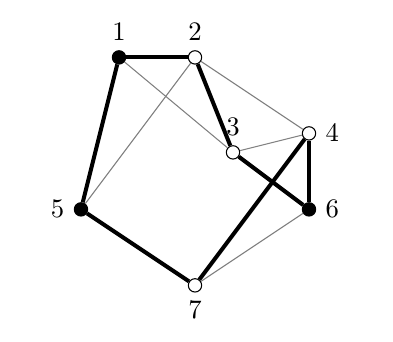
\includegraphics[width=0.4\textwidth]{ejemplo_0.png}
    \caption{Una instancia con B = \textbraceleft 1, 5, 6\textbraceright, W = \textbraceleft 2, 3, 4, 7\textbraceright, y una solución factible indicada por las aristas gruesas para Q = 2 y L = 3. La solución es óptima, por ejemplo, cuando el costo y la distancia de cada arista es 1 para todas las contenidas en la solución, y 2 para el resto.}
    \label{fig:ejemplo_0}
\end{figure}

Entre las aplicaciones de este problema están las operaciones aéreas de trayectos cortos. En este caso los vértices negros pueden representar estaciones de mantenimiento que los aviones tienen que visitar después de Q + 1 tramos como máximo, o después de haber recorrido una distancia máxima de L.

BWTSP es un problema NP-Hard por lo que es atacado mediantes optimización combinatoria para encontrar soluciones exactas.

\subsection{Terminología}

\theoremstyle{definition}
\begin{definition}{Región Factible}

  Una Región Factible es el conjunto de las \textit{soluciones factibles}, es decir, el conjunto de todos los posibles puntos (conjuntos de variables) que satisfacen las restricciones del problema.
\end{definition}

\theoremstyle{definition}
\begin{definition}{Función Objetivo}
  
  En problemas de optimización combinatoria, buscamos minimizar (o maximizar) una función $f(x)$ de variables $(x_1,\dots,x_n)$ sobre una región factible $S$ :
  $$min_{x \in S} f(x)$$
  Llamamos a $f(x)$ la función objetivo.
\end{definition}


\theoremstyle{definition}
\begin{definition}{Relajación Lineal}
  
La técnica de relajación linear en un problema de programación lineal entera consiste en ignorar temporalmente la restricción de tener variables enteras.
Por ejemplo, en programa entero 0-1, las restricciones tienen la pinta:
$$x_i \in \{0,1\}$$
La relajación lineal del problema usa las siguientes restricciones:
$$0 \leq x_i \leq 1$$
La técnica de relajación convierte un problema de optimización NP-Hard en un problema relacionado que puede ser resuelto en tiempo polinomial. La solución obtenida con la relajación puede ser usada para ganar información sobre el problema original. 

\end{definition}



\subsection{Branch and Cut}
Branch and cut es un método de optimización combinatoria para resolver problemas de programación lineal entera, en particular, es el método utilizado en el paper estudiado.
La idea detrás de este método, es usar una combinación del método de \textit{planos de corte} con algoritmos de \textit{branch-and-bound}. Estos métodos, funcionan resolviendo una secuencia de \textit{relajaciones lineales} del problema en enteros.
\subsection{Planos de corte}
La idea detrás del método de planos de corte es ir agregando restricciones a un programa lineal hasta que la solución óptima factible tenga valores enteros. Por supuesto, teniendo cuidado con las restricciones que se añaden para que no cambie el problema.
Llamaremos a las restricciones que se añaden, \textit{cortes}. Un corte relativo a una solución fraccional actual, debe satisfacer las siguientes condiciones,
\begin{itemize}
  \item Toda solución entera factible debe ser factible con el corte
  \item La solución fraccionaria actual no debe ser factible con el corte
\end{itemize}

En la figura \ref{fig:ejemplo_cut} se puede ver un ejemplo gráfico de un corte. El círculo rojo representa la solución óptima fraccionaria encontrada. Los círculos negros son las soluciones enteras y la línea roja representa un corte que cumple con ambos requisitos, acotando nuestro espacio de soluciones factibles.
\begin{figure}[H]
  \centering
  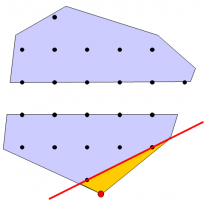
\includegraphics[width=0.4\textwidth]{ejemplo_cut.png}
  \caption{La linea roja representa un corte posible en una instancia.}
  \label{fig:ejemplo_cut}
\end{figure}

Hay dos formas de generar cortes. La primera, los cortes de Gomory genera cortes para cualquier problema de programación lineal. Esta tiene la ventaja de "resolver" cualquier problema, pero la desventaja de que puede ser muy lento. El segundo enfoque, consiste en utilizar la estructura del problema que se quiere resolver para conseguir buenos cortes. De esta forma se pueden conseguir resultados muy buenos pero con la desventaja de tener que hacer un análisis para cada problema por separado.\\

\subsection{Branch and Bound}
El métofo Branch \& Bound (B\&B) es una de las principales herramientas en la construcción de soluciones exactas para problemas de optimización NP-Hard.
Un algoritmo B\&B busca la solución en el espacio de soluciones completo de un problema. Sin embargo, hacer una numeración explicita de las soluciones es imposible debido al exponencialmente creciente número de posibles soluciones.
El uso de cotas combinadas con el valor de la mejor solución actual, permite al algoritmo buscar partes de la solución implicitamente.
En cualquier punto durante el proceso de solucionar el problema, el estado de la solución con respecto a la búsqueda del espacio de soluciones es descripto por una serie de subconjuntos inexplorados del espacio de soluciones junto con la mejor solución encontrada hasta el momento.
Inicialmente, solo un subconjunto existe (el espacio de solución completo) y la mejor solución hayada es $\infty$. Los subespacios no explorados se representan como nodos en un árbol de búsqueda generado dinámicamente, que inicialmente solo contiene la raiz. En cada paso de una iteración de B\&B se procesa un nodo.
 La iteración tiene tres compenentes principales:
 \begin{itemize}
  \item Selección de nodo a procesar.
  \item Calculo de cotas (bound)
  \item Ramificación (branching)
 \end{itemize}

 En la figura \ref{fig:ejemplo_bandb} la situación inicial y el primer paso de un proceso de B\&B es ilustrado.

 El orden en que los componentes de la iteración son ejecutados puede variar según la estrategia utilizada para seleccionar el siguiente nodo a procesar.
 Si la selección del siguiente subproblema está basada en el valor de la cota de los subproblemas, entonces la primera operación en una iteración luego de elegir un nodo es ramificar.
 Por ejemplo, en una subdivisión del espacio de solución de un nodo en dos o mas subespacios a ser investigados en iteraciónes posteriores.
 Para cada uno de estos, se revisa si el subespacio consiste de una sola solución en cuyo caso se compara con la mejor solución actual y se guarda la mejor.
 Si se puede establecer que el subespacio no contiene la solución óptima, se descarta. En caso contrario, se guarda con los nodos a revisar junto con su cota.
 

 
 
 
 \begin{figure}[H]
  \centering
  \includegraphics[width=1.0\textwidth]{ejemplo_bandb.png}
  \caption{Ilustración del espacio de búsqueda de Branch and Bound}
  \label{fig:ejemplo_bandb}
\end{figure}

\section{Modelos}


\begin{align} 
	\min & \sum_{e \in E} c_{e} x_{e} & \label{eq:1} \\
	\text {tal que} & \quad x(\delta(i))=2 & \forall i \in V \label{eq:2} \\
	& x(E(S)) \geq 2 & \forall S \subseteq V \backslash\{1\},\ S \neq \emptyset \label{eq:3} \\
	& \left\{e \in E : x_{e}=1\right\} & \text { satisface la restricción de salto para el camino después de cada } k \in B \label{eq:4} \\
	& \left\{e \in E : x_{e}=1\right\} & \text { satisface la restricción de distancia para el camino después de cada } k \in B \label{eq:5} \\
	& \mathbf{x} \in\{0,1\}^{|E|} & \label{eq:6}
\end{align}

\section{Modelo de porción del camino}

Hasta ahora solamente habíamos comentado un modelo base teórico, con restricciones abstractas que en la práctica deberían reemplazarse. En esta sección introducimos una formulación que se basa en la descripción del problema para determinar las restricciones abstractas. La idea de este modelo es identificar el camino desde un nodo $k \in B$ hasta el nodo negro siguiente sin indicar explícitamente cuál es. A este trayecto nos vamos a referir como “el camino asociado con el nodo $k$". Las variables $x_{i j}^{k} \in\{0,1\},\ \forall k \in B,\ \forall(i, j) \in A$ indican que la arista $(i,j)$ está contenida en la porción del camino general asociada al vértice negro $k$. Con estas variables podemos modelar la porción del camino asociada a cada nodo negro en las restricciones \ref{eq:7}–\ref{eq:10}, al igual que modelar las restricciones de salto y distancia, \ref{eq:4} y \ref{eq:5} respectivamente. A lo largo de este trabajo vamos a explicar en detalle las ecuaciones después de introducirlas.

\begin{align} 
	& x^{k}\left(\delta^{+}(k)\right)=1 & \forall k \in B \label{eq:7} \\
	& \sum_{j \in B \backslash\{k\}} x^{j}\left(\delta^{-}(k)\right)=1 & \forall k \in B \label{eq:8} \\
	& x^{k}\left(\delta^{-}(i)\right)=x^{k}\left(\delta^{+}(i)\right) & \forall k \in B,\ \forall i \in W \label{eq:9} \\
	& \sum_{k \in B} x_{i j}^{k}+x_{j i}^{k}=x_{e} & \forall e=\{i, j\} \in E \label{eq:10}
\end{align}

La ecuación \ref{eq:7} asegura que desde cada nodo negro sale una sola arista y que es parte de su porción del camino. Mientras que la ecuación \ref{eq:8} garantiza que hacia cada nodo de $B$ llega una sola arista, y es parte de la porción del camino de un único nodo negro. Las restricciones de \ref{eq:9} indican que si la arista que llega a un nodo blanco pertenece al camino del nodo negro $k$ entonces la arista que sale de él también, y si no pertenece la que llega entonces la que parte tampoco. Por último, las restricciones \ref{eq:10} unen los dos conjuntos de variables: $x_{e}$ y $x_{i j}^{k}$, expresando que $(i,j)$ o $(j,i)$ son parte de la porción de algún $k$ sí y sólo sí la arista $e$ pertenece al camino final. Para que la formulación sea válida también hay que incluir las restricciones de salto y distancia, \ref{eq:11} y \ref{eq:12} en este caso.

\begin{align} 
	& \sum_{e=\{i, j\} \in E}\left(x_{i j}^{k}+x_{j i}^{k}\right) \leq Q+1 & \forall k \in B \label{eq:11} \\
	& \sum_{e=\{i, j\} \in E} d_{e}\left(x_{i j}^{k}+x_{j i}^{k}\right) \leq L & \forall k \in B \label{eq:12}
\end{align}

Llamamos PS, por \textit{path segment}, a la formulación resultante de reemplazar las restricciones abstractas \ref{eq:4} y \ref{eq:5} por \ref{eq:7}–\ref{eq:12} y las correspondientes a la definición de $x_{i j}^{k}$.

En el trabajo original también se incluye la restricción \ref{eq:13} que relaciona los trayectos asociados a cada nodo negro:

\begin{align}
	& x^{k}\left(\delta^{-}(j)\right)+x^{j}\left(\delta^{-}(k)\right) \leq 1 & \forall k \neq j \in B \label{eq:13}
\end{align}

Esta restricción elimina ciclos al asegurar que si un nodo negro $j$ es el nodo negro inmediatamente siguiente a $k$ de $B$, entonces $k$ no puede estar inmediatamente después de $j$. Los resultados computacionales, que se introducen dentro de algunas secciones, muestran que estas desigualdades mejoran las cotas de PS para algunas instancias evaluadas, y a la variante del modelo que incluye \ref{eq:13} se la llama PS+.

\section{Formulaciones dependientes de la posición}

\subsection{Formulación pura}

\begin{align}
	& X^{1}\left(\delta^{+}(k)\right)=1 & \forall k \in B \label{eq:14} \\
	& \sum_{p=1}^{Q+1} X^{p}\left(\delta^{-}(k)\right)=1 & \forall k \in B \label{eq:15} \\
	& X^{p}\left(\delta^{-}(i)\right)=X^{p+1}\left(\delta^{+}(i)\right) & \forall i \in W,\ \forall p \in\{1,2, \ldots, Q\} \label{eq:16} \\
	& \sum_{p=1}^{Q+1}\left(X_{i j}^{p}+X_{j i}^{p}\right)=x_{e} & \forall e=\{i, j\} \in E \label{eq:17}
\end{align}

\begin{align}
	& \sum_{e \in P} x_{e} \leq|P|-1 & \forall P \in \mathcal{P}_{\mathrm{inf}} \label{eq:18}
\end{align}

\begin{align}
	& X_{i j}^{p} \leq \sum_{h \neq i} X_{j h}^{p+1} & \forall p \in\{1,2, \ldots, Q\},\ \forall e=\{i, j\} \in E, j \in W \label{eq:19} \\
	& X_{i j}^{p} \leq \sum_{h \neq i} X_{j h}^{1} & \forall p \in\{1,2, \ldots, Q+1\},\ \forall e=\{i, j\} \in E, j \in B \label{eq:20}
\end{align}

\begin{align}
	& X\left(\delta^{-}(S)\right) \geq 1 & \forall S \subseteq V_{\mathrm{Q}} \backslash\left\{j_{0} : j \in B\right\}, \exists i \in W |\left\{i_{p}, p \in\{1,2, \ldots, Q\}\right\} \subseteq S \label{eq:21}
\end{align}

\subsection{Formulación de una porción del camino}

(Modelos traducidos así nomás. Hay que mejorar seguro este)

\begin{align}
	& Y^{k, 1}\left(\delta^{+}(k)\right)=1 & \forall k \in B \label{eq:22} \\
	& \sum_{j \in B \backslash\{k\}} \sum_{p=1}^{Q+1} Y^{j, p}\left(\delta^{-}(k)\right)=1 & \forall k \in B \label{eq:23} \\
	& Y^{k, p}\left(\delta^{-}(i)\right)=Y^{k, p+1}\left(\delta^{+}(i)\right) & \forall k \in B, \forall i \in W, \forall p \in\{1, \ldots, Q\} \label{eq:24} \\
	& \sum_{k \in B} \sum_{p=1}^{Q+1}\left(Y_{i j}^{k, p}+Y_{j i}^{k, p}\right)=x_{e} & \forall e=\{i, j\} \in E \label{eq:25}
\end{align}

\begin{align}
	& \sum_{p=1}^{Q+1} \sum_{e=\{i, j\} \in E} d_{e}\left(Y_{i j}^{k, p}+Y_{j i}^{k, p}\right) \leq L & \forall k \in B \label{eq:26}
\end{align}

\begin{align}
	& Y_{i j}^{k, p} \leq \sum_{h \neq i} Y_{j h}^{k, p+1} & \forall k \in B,\ \forall p \in\{1,2, \ldots, Q\}, \forall e=\{i, j\} \in E, j \in W \label{eq:27} \\
	& Y_{i j}^{k, p} \leq \sum_{h \neq i} Y_{j h}^{j, 1} & \forall k \in B,\ \forall p \in\{1,2, \ldots, Q+1\}, \forall e=\{i, j\} \in E, j \in B \backslash\{k\} \label{eq:28}
\end{align}

\begin{align}
	& Y\left(\delta^{-}(S)\right) \geq 1 & \forall S \subseteq V_{\mathrm{QB}} \backslash\{j_{0}^{j} : j \in B\},\ \exists i \in W |\left\{i_{p}^{k}, k \in B, p \in\{1,2, \ldots, Q\}\right\} \subseteq S \label{eq:29}
\end{align}

\subsection{Modelo 2-dimensional}

\begin{align}
	& Z^{1,1}\left(\delta^{+}(1)\right)=1 \label{eq:30} \\
	& \sum_{j \in B \backslash\{1\}} Z^{m, 1}\left(\delta^{+}(j)\right)=1 & \forall m \in\{2,3, \ldots,|B|\} \label{eq:31} \\
	& \sum_{i \in V \backslash\{1\}} \sum_{p=1}^{Q+1} \sum_{p=1} \sum_{i 1}^{|B|, p}=1 \label{eq:32} \\
	& \sum_{i \in V} \sum_{p=1}^{Q+1} \sum_{p=1} Z_{i k}^{m, p}=1 & \forall m \in\{2,3, \ldots,|B|\},\ \forall k \in B \backslash\{1\} \label{eq:33} \\
	& Z^{m, p}\left(\delta^{-}(i)\right)=Z^{m, p+1}\left(\delta^{+}(i)\right) & \forall m \in\{1,2, \ldots,|B|\}, \forall p \in\{1,2, \ldots, Q\},\ \forall i \in W \label{eq:34} \\
	& \sum_{m=1}^{|B|} \sum_{p=1}^{Q+1}\left(Z_{i j}^{m, p}+Z_{j i}^{m, p}\right)=x_{e} & \forall e=\{i, j\} \in E \label{eq:35}
\end{align}

\begin{align}
	& \sum_{p=0}^{Q} \sum_{e=\{i, j\} \in E} d_{e}\left(Z_{i j}^{m, p}+Z_{j i}^{m, p}\right) \leq L \quad \forall m \in\{1,2, \ldots,|B|\} \label{eq:36}
\end{align}

\begin{align}
	& Z_{i j}^{m, p} \leq \sum_{h \neq i} Z_{j h}^{m, p+1} & \forall m \in\{1,2, \ldots,|B|\},\ \forall p \in\{1,2, \ldots, Q\},\ \forall e=\{i, j\} \in E, j \in W \label{eq:37} \\
	& Z_{i j}^{m, p} \leq \sum_{h \neq i} Z_{j h}^{m+1,1} & \forall m \in\{1,2, \ldots,|B|-1\},\ \forall p \in\{1,2, \ldots, Q+1\},\ \forall e=\{i, j\} \in E, j \in B \backslash\{1\} \label{eq:38} \\
	& Z_{i 1}^{|B|, p} \leq \sum_{h \neq i} Z_{1 h}^{1,1} & \forall p \in\{1,2, \ldots, Q+1\},\ \forall e=\{i, 1\} \in E \label{eq:39}
\end{align}

\begin{multline}
	 Z(\delta^{-}(S)) \geq 1 \quad \quad \forall S \subseteq V_{\mathrm{QI}} \backslash\{i_{0}^{m} | i \in B, m \in\{1,2, \ldots,|B|\}, \\
	 \exists i \in W : \{i_{p}^{m} | p \in \{1,2, \ldots, Q\}, m \in \{1,2, \ldots,|B|\}\} \subseteq S \label{eq:40}
\end{multline}

\section{Modelos alternativos dependientes del tiempo}

\section{Comparaciones teóricas}

\subsection{Pre-procesamiento}

\subsection{Algoritmo de plano de corte}

\subsection{Heurísticas}

\section{Resultados empíricos}

(Por ahí habría que mejorar este título)

\subsection{Instancias}

\subsection{Relajaciones}

\subsection{Análisis de los resultados}

\pagebreak

\begin{thebibliography}{9}

\bibitem{main}
L. Gouveia, M. Leitner y M. Ruthmair, “Extended formulations and branch-and-cut algorithms for the Black-and-White Traveling Salesman Problem". European Journal of Operational Research, 262-3, 908-928. 2017.

\bibitem{ip_tutorial}
G. Cornuéjols, M. Trick y M. Saltzman, “A tutorial on integer programming". CMU Technical Report. 1995.

\bibitem{teaching_ip_tsp}
G. Pataki, “Teaching integer programming formulations using the traveling salesman problem". SIAM Review 45-1, 116-123. 2003.

\bibitem{branch_and_cut}
J. E. Mitchell, “Branch-and-Cut Algorithms for Combinatorial Optimization Problems". 2002.

\bibitem{branc_and_bound}
J. Clausen, “Branch and Bound Algorithms—Principles and Examples". 1999.

\end{thebibliography}

\end{document}